\documentclass[tikz,border=10pt]{standalone}
\usepackage{bm}
\usepackage{mathrsfs}
\begin{document}
  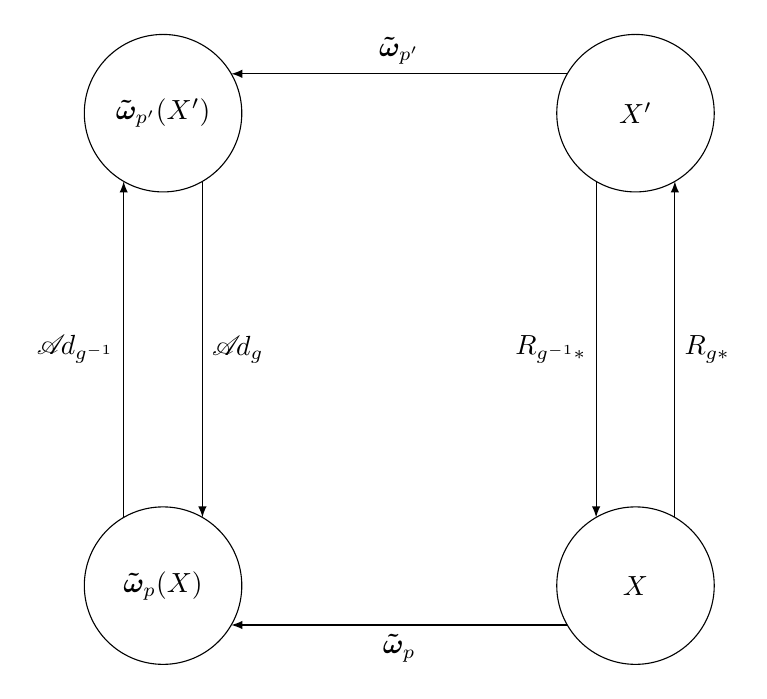
\begin{tikzpicture}
  \draw (-3,-3) circle (1) node {$\bm{\tilde{\omega}}_p(X)$};
  \draw (3,-3) circle (1) node {$X$};
  \draw (3,3) circle (1) node {$X'$};
  \draw (-3,3) circle (1) node {$\bm{\tilde{\omega}}_{p'}(X')$};
  \draw[-latex] ({3+1*cos(60)}, {-3 + 1*sin(60)}) -- ({3+1*cos(60)},{3 - 1 * sin(60)}) node[pos = 0.5,right]{$R_{g*}$};
  \draw[latex-] ({3-1*cos(60)}, {-3 + 1*sin(60)}) -- ({3-1*cos(60)},{3 - 1 * sin(60)}) node[pos = 0.5,left]{$R_{g^{-1}*}$};
  \draw[-latex] ({3+1*cos(150)}, {3 + 1*sin(150)}) -- ({-3+1*cos(30)},{3 + 1 * sin(30)}) node[pos = 0.5,above]{$\bm{\tilde{\omega}}_{p'}$ } ;
  % \draw[latex-] ({3+1*cos(-150)}, {3 + 1*sin(-150)}) -- ({-3+1*cos(-30)},{3 + 1 * sin(-30)}) node[pos = 0.5,below]{$\bm{\tilde{\omega}}_{p'}^{-1}$} ;
  \draw[-latex] ({-3-1*cos(60)}, {-3 + 1*sin(60)}) -- ({-3-1*cos(60)},{3 - 1 * sin(60)}) node[pos = 0.5,left]{$\mathscr{A}\!d_{g^{-1}}$};
  \draw[latex-] ({-3+1*cos(60)}, {-3 + 1*sin(60)}) -- ({-3+1*cos(60)},{3 - 1 * sin(60)}) node[pos = 0.5,right ]{$\mathscr{A}\!d_{g}$};
  \draw[-latex]  ({3+1*cos(-150)}, {-3 + 1*sin(-150)}) -- ({-3+1*cos(-30)},{-3 + 1 * sin(-30)}) node[pos = 0.5,below]{$\bm{\tilde{\omega}}_{p}$ } ;
  % \draw[latex-] ({3+1*cos(150)}, {-3 + 1*sin(150)}) -- ({-3+1*cos(30)},{-3 + 1 * sin(30)}) node[pos = 0.5,above ]{$\bm{\tilde{\omega}}_{p}^{-1}$} ;
\end{tikzpicture}
\end{document}
